\documentclass[11pt, a4paper]{article}

% ── Packages ──────────────────────────────────────────────────────────────────
\usepackage[margin=2.5cm]{geometry}
\usepackage{amsmath, amssymb, amsthm}
\usepackage{bm}
\usepackage{graphicx}
\usepackage{xcolor}
\usepackage{booktabs}
\usepackage{array}
\usepackage{tikz}
\usetikzlibrary{arrows.meta, positioning, shapes.geometric, fit, backgrounds, calc}
\usepackage{algorithm}
\usepackage{algpseudocode}
\usepackage{hyperref}
\usepackage{enumitem}
\usepackage{mdframed}
\usepackage{caption}
\usepackage{subcaption}

% ── Colours ───────────────────────────────────────────────────────────────────
\definecolor{aifblue}{RGB}{30, 90, 180}
\definecolor{aifgreen}{RGB}{0, 140, 80}
\definecolor{aifgray}{RGB}{90, 90, 90}
\definecolor{aifred}{RGB}{180, 40, 40}
\definecolor{aifpurple}{RGB}{120, 40, 160}
\definecolor{boxbg}{RGB}{240, 246, 255}
\definecolor{warningbg}{RGB}{255, 248, 230}
\definecolor{notefg}{RGB}{50, 80, 160}

% ── Custom environments ────────────────────────────────────────────────────────
\newmdenv[
  backgroundcolor=boxbg,
  linecolor=aifblue,
  linewidth=1.5pt,
  roundcorner=4pt,
  innertopmargin=8pt,
  innerbottommargin=8pt
]{keybox}

\newmdenv[
  backgroundcolor=warningbg,
  linecolor=orange,
  linewidth=1.5pt,
  roundcorner=4pt,
  innertopmargin=8pt,
  innerbottommargin=8pt
]{notebox}

% ── Macros ─────────────────────────────────────────────────────────────────────
\newcommand{\vect}[1]{\bm{#1}}
\newcommand{\mat}[1]{\mathbf{#1}}
\newcommand{\FE}{\mathcal{F}}
\newcommand{\Pip}{\mat{\Pi}_p}
\newcommand{\Pis}{\mat{\Pi}_s}
\newcommand{\epsp}{\vect{\varepsilon}_p}
\newcommand{\epss}{\vect{\varepsilon}_s}

% ── Title ──────────────────────────────────────────────────────────────────────
\title{%
  \textbf{\Large Continuous Active Inference for 3-D Trajectory Tracking}\\[4pt]
  \large Algorithm Description \& Mathematical Framework
}
\author{}
\date{}

% ══════════════════════════════════════════════════════════════════════════════
\begin{document}
\maketitle
\thispagestyle{empty}
\vspace{-1em}
\tableofcontents
\newpage

% ══════════════════════════════════════════════════════════════════════════════
\section{Overview}

This document describes a \textbf{continuous-time Active Inference} (AIF) agent
that tracks a 3-D trajectory under gravity. The system illustrates a key
principle of the Free Energy Principle: axes that are \emph{neither observed nor
modelled} accumulate unbounded uncertainty and drift --- the agent cannot and
does not attempt to correct them.

\begin{keybox}
\textbf{Core design asymmetry.}
\begin{itemize}[noitemsep]
  \item \textbf{$x$-axis} (horizontal): controlled $+$ visual feedback.
  \item \textbf{$y$-axis} (vertical): controlled $+$ proprioceptive / visual feedback;
        gravity compensation built in.
  \item \textbf{$z$-axis} (depth): \emph{uncontrolled, no feedback} --- undergoes
        a random walk driven by unmodelled noise.
\end{itemize}
\end{keybox}

% ══════════════════════════════════════════════════════════════════════════════
\section{State \& Action Spaces}

\subsection{State vector}
The full state is
\begin{equation}
  \vect{x} = \bigl[p_1,\; p_2,\; p_3,\; v_1,\; v_2,\; v_3\bigr]^\top \in \mathbb{R}^6,
\end{equation}
where $(p_1, p_2, p_3)$ are positions along $(x, y, z)$ and
$(v_1, v_2, v_3)$ the corresponding velocities.

\subsection{Action vector}
\begin{equation}
  \vect{a} = [u_1,\; u_2]^\top \in \mathbb{R}^2, \qquad u_3 \equiv 0.
\end{equation}
No action is generated along $z$ because the free-energy gradient
$\partial\FE/\partial u_3 = 0$ (Sec.~\ref{sec:fe}).

% ══════════════════════════════════════════════════════════════════════════════
\section{Generative Process (True World)}
\label{sec:gp}

The continuous-time dynamics of the real world are
\begin{align}
  \dot{p}_1 &= v_1, & \dot{p}_2 &= v_2, & \dot{p}_3 &= v_3,\\[4pt]
  \dot{v}_1 &= \frac{u_1}{m_1} + \omega_x(t), &
  \dot{v}_2 &= \frac{u_2}{m_2} - g + \omega_y(t), &
  \dot{v}_3 &= \omega_z(t),
\end{align}
where $g = 9.81\;\text{m/s}^2$ and $\omega_i$ are independent Gaussian white-noise
processes,
\begin{equation}
  \omega_i(t) \sim \mathcal{N}\!\left(0,\;\frac{\sigma_i^2}{\Delta t}\right), \quad i\in\{x,y,z\}.
\end{equation}

\begin{notebox}
\textbf{Why $z$ drifts.}
Because $\dot{v}_3 = \omega_z(t)$ and $u_3 = 0$, the $z$-velocity performs
a Wiener process (Brownian motion) with diffusion coefficient $\sigma_z$:
\[
  v_3(t) = v_3(0) + \int_0^t \omega_z(s)\,\mathrm{d}s,\qquad
  \operatorname{Var}[v_3(t)] = \sigma_z^2 t.
\]
Integrating once more, $p_3$ follows a second-order random walk.
This mimics the inertia-induced depth drift observed in arm-movement experiments.
\end{notebox}

\paragraph{Observation model.}
Only the $x$-$y$ components are sensed:
\begin{equation}
  \vect{y}_{\text{obs}} = \bigl[p_1, p_2, \underbrace{-}_{?}, v_1, v_2, \underbrace{-}_{?}\bigr]^\top
    + \vect{\eta}, \quad
  \vect{\eta}\sim\mathcal{N}(\mathbf{0}, \mat{\Sigma}_{\text{obs}}),
\end{equation}
where $-$ denotes unobserved entries; in practice those slots are set equal to
the current belief $\vect{\mu}$ so that the sensory prediction error on $z$
is identically zero.

% ══════════════════════════════════════════════════════════════════════════════
\section{Generative Model (Agent's Internal Model)}
\label{sec:gm}

The agent assumes $z$ is \emph{stationary}:
\begin{align}
  f_{\text{model},\,p_3}(\vect{x},\vect{a}) &= 0, \\
  f_{\text{model},\,v_3}(\vect{x},\vect{a}) &= 0.
\end{align}
For the controlled axes the model mirrors the true physics:
\begin{equation}
  \vect{f}_{\text{model}}(\vect{x},\vect{a})
  = \bigl[v_1,\;v_2,\;0,\;u_1/m_1,\;u_2/m_2 - g,\;0\bigr]^\top.
\end{equation}
Combined with $\Pi_{s,z}=0$ (no $z$-observations), the belief about $z$
is completely frozen at its initial value --- the agent \emph{correctly} does
nothing about a dimension it cannot observe or model.

\subsection{Prior / Reference trajectory}
\begin{equation}
  \vect{x}^*(t) = \bigl[p_1^*(t),\;p_2^*,\;0,\;v_1^*,\;0,\;0\bigr]^\top,
\end{equation}
with a linear ramp in $x$:
\begin{equation}
  p_1^*(t) = x_{\text{start}} + (x_{\text{end}} - x_{\text{start}})\,
             \min\!\left(\tfrac{t}{T_{\text{end}}},1\right).
\end{equation}

% ══════════════════════════════════════════════════════════════════════════════
\section{Free Energy \& Precision Matrices}
\label{sec:fe}

\subsection{Variational free energy}
\begin{equation}
  \FE(\vect{\mu}, \vect{a}) = \underbrace{\tfrac{1}{2}\,\epsp^\top\,\Pip\,\epsp}_{\text{prior cost}}
                            + \underbrace{\tfrac{1}{2}\,\epss^\top\,\Pis\,\epss}_{\text{sensory cost}},
\end{equation}
where the prediction errors are
\begin{equation}
  \epsp = \vect{\mu} - \vect{x}^*(t), \qquad
  \epss = \vect{y}_{\text{obs}} - \vect{\mu}.
\end{equation}

\subsection{Precision matrices}
Both $\Pip$ and $\Pis$ are $6\times 6$ diagonal matrices with structure:

\begin{equation}
  \Pis = \operatorname{diag}\!\left(
    \tfrac{1}{\sigma_{s,\text{pos}}^2},\;
    \tfrac{1}{\sigma_{s,\text{pos}}^2},\;
    \mathbf{0},\;
    \tfrac{1}{\sigma_{s,\text{vel}}^2},\;
    \tfrac{1}{\sigma_{s,\text{vel}}^2},\;
    \mathbf{0}
  \right),
\end{equation}
\begin{equation}
  \Pip = \operatorname{diag}\!\left(
    \tfrac{1}{\sigma_{p,\text{pos}}^2},\;
    \tfrac{1}{\sigma_{p,\text{pos}}^2},\;
    \tfrac{1}{\sigma_{p,z}^2}\!\approx\!0,\;
    \tfrac{1}{\sigma_{p,\text{vel}}^2},\;
    \tfrac{1}{\sigma_{p,\text{vel}}^2},\;
    \tfrac{1}{\sigma_{p,z}^2}\!\approx\!0
  \right).
\end{equation}

\begin{keybox}
\textbf{Why no $z$-action is generated.}
The action gradient
$\partial\FE/\partial u_3$
involves $\Pis\,\epss$ and $\Pip\,\epsp$ projected onto the $z$-rows.
Since $\Pi_{s,z} = 0$ (zero sensory precision on $z$) and $\Pi_{p,z}\approx 0$
(negligible prior precision on $z$), this gradient is identically zero:
\[
  \frac{\partial \FE}{\partial u_3} = 0 \quad\Rightarrow\quad u_3 \equiv 0.
\]
\end{keybox}

% ══════════════════════════════════════════════════════════════════════════════
\section{Belief Update (Perception)}

The agent's belief $\vect{\mu}$ is updated by gradient descent on free energy,
corrected by the model's own flow:
\begin{equation}
  \dot{\vect{\mu}} = \vect{f}_{\text{model}}(\vect{\mu}, \vect{a})
                    + \kappa_\mu \bigl(\Pis\,\epss - \Pip\,\epsp\bigr),
\end{equation}
with learning rate $\kappa_\mu > 0$. The first term propagates the belief
forward according to the agent's dynamics; the bracketed term drives the
belief towards the observation (sensory term) and away from the prior error
(prior term).

\paragraph{$z$-axis behaviour.}
For the $z$-components:
\begin{itemize}[noitemsep]
  \item $f_{\text{model},z} = 0$ (stationary model assumption),
  \item $\Pi_{s,z}\,\varepsilon_{s,z} = 0$ (no $z$-observation),
  \item $\Pi_{p,z}\,\varepsilon_{p,z} \approx 0$ (weak $z$-prior).
\end{itemize}
Hence $\dot{\mu}_z \approx 0$: the $z$-belief is frozen.

% ══════════════════════════════════════════════════════════════════════════════
\section{Action Policy (Active Inference)}

The control law minimises $\FE$ with respect to $\vect{a}$.
Because the sensory precision on $z$ is zero, this reduces to a PD
controller on the $x$-$y$ plane only:

\begin{align}
  u_1 &= m_1\bigl[K_P\,(p_1^* - p_1) + K_D\,(v_1^* - v_1)\bigr], \\[4pt]
  u_2 &= m_2\bigl[K_P\,(p_2^* - p_2) + K_D\,(v_2^* - v_2)\bigr] + m_2 g,
\end{align}
clipped to $[-a_{\max}, a_{\max}]$. The gravity feed-forward term $m_2 g$ in
$u_2$ emerges naturally from including $g$ in the generative model.

% ══════════════════════════════════════════════════════════════════════════════
\section{Algorithm}

\begin{algorithm}[H]
\caption{Continuous Active Inference --- 3-D Trajectory Tracking}
\label{alg:aif}
\begin{algorithmic}[1]
\Require Parameters $\{m_1, m_2, g, K_P, K_D, \kappa_\mu, \Delta t, T_{\text{end}}\}$,
         precision matrices $\Pip$, $\Pis$,
         noise levels $\{\sigma_x, \sigma_y, \sigma_z\}$
\State \textbf{Initialise:} $\vect{x}_{\text{real}} \leftarrow \vect{x}_0$;\quad
       $\vect{\mu} \leftarrow \vect{x}_0$
\State Pre-draw noise arrays:
       $\omega_i[k] \sim \mathcal{N}(0,\,\sigma_i^2/\Delta t)$
       for $i \in \{x,y,z\}$, $k = 0,\ldots,N-1$
\For{$k = 0, 1, \ldots, N-1$}
  \State $t \leftarrow k\,\Delta t$
  \State \textbf{Reference:} $\vect{x}^*(t) \leftarrow$ \Call{DesiredState}{$t$}
  \State
  \State \textbf{--- Perception ---}
  \State Observe $\vect{y}_{\text{obs}}$: set $y_{p_3} \leftarrow \mu_{p_3}$,
         $y_{v_3} \leftarrow \mu_{v_3}$
         \quad($\Rightarrow \varepsilon_{s,z} = 0$)
  \State Compute prediction errors:
         $\epsp \leftarrow \vect{\mu} - \vect{x}^*$;\quad
         $\epss \leftarrow \vect{y}_{\text{obs}} - \vect{\mu}$
  \State Compute free energy:
         $\FE \leftarrow \tfrac12 \epsp^\top\!\Pip\epsp + \tfrac12 \epss^\top\!\Pis\epss$
  \State
  \State \textbf{--- Action ---}
  \State $u_1 \leftarrow m_1[K_P(p_1^* - \mu_{p_1}) + K_D(v_1^* - \mu_{v_1})]$
  \State $u_2 \leftarrow m_2[K_P(p_2^* - \mu_{p_2}) + K_D(v_2^* - \mu_{v_2})] + m_2 g$
  \State Clip $u_1, u_2 \in [-a_{\max}, a_{\max}]$;\quad $u_3 \leftarrow 0$
  \State
  \State \textbf{--- World update ---}
  \State $\dot{\vect{x}}_{\text{real}} \leftarrow
         \vect{f}_{\text{proc}}(\vect{x}_{\text{real}}, \vect{a},
                                [\omega_x[k],\omega_y[k],\omega_z[k]])$
  \State $\vect{x}_{\text{real}} \leftarrow \vect{x}_{\text{real}} + \dot{\vect{x}}_{\text{real}}\,\Delta t$
  \State
  \State \textbf{--- Belief update ---}
  \State $\dot{\vect{\mu}} \leftarrow
         \vect{f}_{\text{model}}(\vect{\mu}, \vect{a})
         + \kappa_\mu\bigl(\Pis\epss - \Pip\epsp\bigr)$
  \State $\vect{\mu} \leftarrow \vect{\mu} + \dot{\vect{\mu}}\,\Delta t$
  \State
  \State Store $\vect{x}_{\text{real}},\,\vect{\mu},\,\vect{x}^*,\,\vect{a},\,\FE$
\EndFor
\end{algorithmic}
\end{algorithm}

% ══════════════════════════════════════════════════════════════════════════════
\section{System Diagram}

\begin{figure}[ht]
\centering
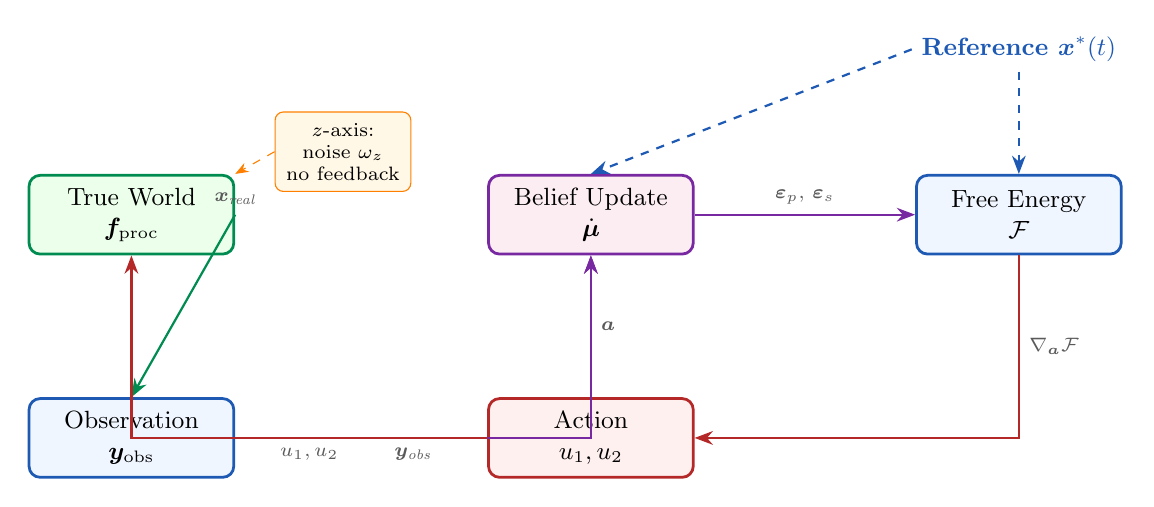
\begin{tikzpicture}[
  node distance = 1.6cm and 2.4cm,
  every node/.style = {font=\small},
  box/.style     = {draw, rounded corners=4pt, minimum height=1.0cm,
                    minimum width=2.6cm, align=center, fill=boxbg,
                    draw=aifblue, line width=1pt},
  worldbox/.style = {box, fill=green!8, draw=aifgreen},
  actionbox/.style= {box, fill=red!6,  draw=aifred},
  beliefbox/.style = {box, fill=purple!7, draw=aifpurple},
  arrow/.style   = {-Stealth, thick},
  dasharrow/.style = {-Stealth, thick, dashed, gray},
  label/.style   = {font=\scriptsize\itshape, color=aifgray}
]

% Nodes
\node[worldbox]  (world)   {True World\\$\vect{f}_{\text{proc}}$};
\node[beliefbox, right=3.2cm of world] (belief) {Belief Update\\$\dot{\vect{\mu}}$};
\node[actionbox, below=1.8cm of belief] (action) {Action\\$u_1, u_2$};
\node[box,        below=1.8cm of world]  (obs)    {Observation\\$\vect{y}_{\text{obs}}$};
\node[box,        right=2.8cm of belief] (fe)     {Free Energy\\$\FE$};

% Arrows
\draw[arrow, aifgreen]
  (world.east) -- node[above, label]{$\vect{x}_{\text{real}}$} (obs.east |- world.east)
  -- (obs.north);

\draw[arrow, aifpurple]
  (obs.east) -- node[below, label]{$\vect{y}_{\text{obs}}$} (belief.south |- obs.east)
  -- (belief.south);

\draw[arrow, aifpurple]
  (belief.east) -- node[above, label]{$\epsp,\,\epss$} (fe.west);

\draw[arrow, aifred]
  (fe.south) -- node[right, label]{$\nabla_{\vect{a}}\FE$}
  (fe.south |- action.east) -- (action.east);

\draw[arrow, aifred]
  (action.west) -- node[below, label]{$u_1, u_2$} (world.south |- action.west) -- (world.south);

\draw[arrow, aifpurple]
  (action.north) -- node[right, label]{$\vect{a}$} (belief.south);

% Reference
\node[above=1.3cm of fe, draw=none, text=aifblue, font=\small\bfseries] (ref)
  {Reference $\vect{x}^*(t)$};
\draw[dasharrow, aifblue] (ref.west) -- (belief.north);
\draw[dasharrow, aifblue] (ref.south) -- (fe.north);

% z-drift annotation
\node[right=0.5cm of world, yshift=0.8cm,
      draw=orange, rounded corners=3pt, fill=warningbg,
      font=\scriptsize, align=center, inner sep=4pt] (zdrift)
  {$z$-axis:\\noise $\omega_z$\\no feedback};
\draw[-Stealth, orange, dashed] (zdrift.west) -- (world.north east);

\end{tikzpicture}
\caption{%
  Active Inference loop. Green: world dynamics; purple: perception/belief;
  red: action policy; orange: uncontrolled $z$-perturbation (no feedback path exists).
}
\label{fig:aif-loop}
\end{figure}

% ══════════════════════════════════════════════════════════════════════════════
\section{Parameter Summary}

\begin{table}[ht]
\centering
\caption{Default simulation parameters.}
\label{tab:params}
\renewcommand{\arraystretch}{1.35}
\begin{tabular}{lll}
\toprule
\textbf{Symbol} & \textbf{Description} & \textbf{Default value} \\
\midrule
$m_1, m_2$         & Effective masses ($x$, $y$)                    & $1.0\;\text{kg}$ \\
$g$                & Gravitational acceleration                       & $9.81\;\text{m/s}^2$ \\
$K_P$              & Proportional gain                                & $20.0$ \\
$K_D$              & Derivative gain                                  & $12.0$ \\
$a_{\max}$         & Action clip bound                                & $50.0\;\text{N}$ \\
$\kappa_\mu$       & Belief learning rate                             & $1.0$ \\
$\Delta t$         & Integration step                                 & $0.01\;\text{s}$ \\
$T_{\text{end}}$   & Episode duration                                 & $4.0\;\text{s}$ \\
\midrule
$\sigma_{s,\text{pos}}$ & Sensory pos.\ precision (x,y)             & $0.1$ \\
$\sigma_{s,\text{vel}}$ & Sensory vel.\ precision (x,y)             & $0.15$ \\
$\sigma_{s,z}$          & Sensory $z$ precision                     & $0$ (unobserved) \\
$\sigma_{p,\text{pos}}$ & Prior pos.\ precision (x,y)               & $0.1$ \\
$\sigma_{p,z}$          & Prior $z$ precision                       & $1.0\gg\sigma_{p,\text{pos}}$ \\
\midrule
$\sigma_z$         & Process noise on $z$-velocity                    & tunable \\
\bottomrule
\end{tabular}
\end{table}

% ══════════════════════════════════════════════════════════════════════════════
\section{Key Properties \& Interpretation}

\begin{enumerate}[leftmargin=*, label=\textbf{\arabic*.}]

\item \textbf{Asymmetric control.}
  The $x$-$y$ plane is fully controlled via PD action derived from free-energy
  minimisation. The $z$-axis is intentionally ignored at every level: no model,
  no observation, no action.

\item \textbf{Gravity compensation.}
  Because gravity appears in both the generative process and the generative
  model, the feed-forward term $m_2 g$ in $u_2$ cancels it exactly, keeping
  $p_2 \approx p_2^*$ at all times.

\item \textbf{Frozen $z$-belief as a correct AIF solution.}
  Setting $\Pi_{s,z}=0$ is not a hack --- it is the principled Bayesian answer
  to ``I have no information about $z$''. The belief update equation then gives
  $\dot{\mu}_z = 0$, so the agent neither tracks nor fights the $z$-drift.

\item \textbf{Free energy as a dual objective.}
  $\FE$ simultaneously encodes trajectory tracking (via $\Pip$, which punishes
  deviations from $\vect{x}^*$) and sensory consistency (via $\Pis$, which
  punishes deviations between observations and belief). Increasing $\Pip$
  relative to $\Pis$ tightens trajectory adherence; increasing $\Pis$ makes
  the agent more reactive to sensory input.

\item \textbf{Extensibility.}
  The framework naturally accommodates:
  \begin{itemize}[noitemsep]
    \item Non-linear or time-varying reference trajectories (replace
          \texttt{desired\_full\_state}).
    \item Salient stimuli: add a salience-weighted term to $\FE$ that attracts
          the reference or modulates $\Pis$ dynamically.
    \item Partial $z$-feedback: simply set $\Pi_{s,z}>0$ and extend
          $\vect{y}_{\text{obs}}$ to include $p_3$; the belief will begin
          tracking and correcting $z$-drift.
  \end{itemize}

\end{enumerate}

% ══════════════════════════════════════════════════════════════════════════════
\appendix
\section{Discrete Integration}

All ODEs are integrated with the forward Euler scheme:
\begin{equation}
  \vect{x}(t+\Delta t) = \vect{x}(t) + \vect{f}\bigl(\vect{x}(t), \vect{a}(t)\bigr)\,\Delta t.
\end{equation}
For the stochastic noise, each sample is scaled as
$\omega_i \sim \mathcal{N}(0,\,\sigma_i^2/\Delta t)$ so that the
\emph{integrated} increment over one step has variance $\sigma_i^2\,\Delta t$,
consistent with a Wiener process of diffusion rate $\sigma_i$.

\end{document}
